\section{Implementation}
%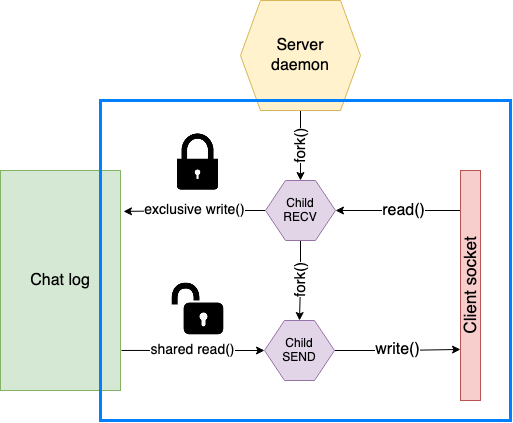
\includegraphics[width=1in,height=1.25in,keepaspectratio]{img/server.png}
\begin{figure}[!t]
	\centering
	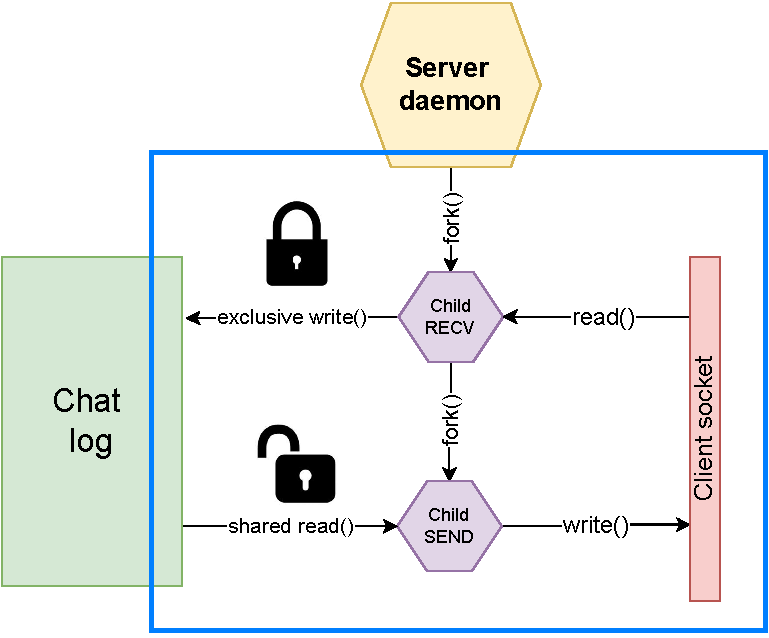
\includegraphics[width=2.5in]{img/server.pdf}
	%where an .eps filename suffix will be assumed under latex, 
	%and a .pdf suffix will be assumed for pdflatex; or what has been declared
	%via \DeclareGraphicsExtensions.
	\caption{Server's back-end architectural overview. The blue rectangle denotes the process cluster created exclusively for each client taking part in a chat service.}
	\label{fig_server_backend}
\end{figure}
The requirements for the chat application are that an undefined number of participants can simultaneously exchange text messages in a chatroom. Furthermore, the communication might be asynchronous, so that the participants can read messages sent to them while they were not connected to the server. The application should use the least amount of dependencies as possible to enable portability across Unix systems, i.e. the chat server should compile natively to FreeBSD or a Linux distribution with the same source file.

The server fundamentally requires a process working as a daemon accepting incoming connection attempts from clients. For each accepted client connection there are multiple possibilities regarding the architecture of the server. The daemon could handle each client separately in a unique thread or child process.

The server will mostly have an IO-bound workload, consisting of handling asynchronous network packets and writing the messages from the users into files in the server's filesystem. An IO-bound workload benefits from the use of a pre-emptive scheduler, since the threads or processes are constantly changing alternatively between a blocked and an unblocked state in an unpredictable manner. As soon as a client goes silent the pre-emptive scheduler can run any other runnable process \cite{Kennedy2018}. Hence, the context-switching is actually advantageous for IO-bound workloads, whereas in CPU-bound workloads (e.g. intensive long-running sequential computations) it becomes a performance bottleneck.

Therefore, handling each client connection separately by forking a child process seems like a good fit for the kind of workload that is expected. Nonetheless, it must be acknowledged that a counterargument against using processes is that thread creation and context-switching times are generally faster than for processes, since processes have an inherently more complex memory layout than threads \cite{Kerrisk2010}.

However, other reasons settled the decision towards processes instead of threads. Before going into these reasons, it makes sense to review the architecture that was actually implemented as a solution. Figure \ref{fig_server_backend} shows a high-level representation of how the server handles every client connection. After successfully authenticating a client, the server daemon calls the \textit{fork} syscall and creates a new child process exclusively for the new client.
 
This child process, called "\textit{Child RECV}" in fig. \ref{fig_server_backend}, inherits a copy of the newly established socket which handles the client. Child RECV is responsible for reading any incoming messages from the client, writing these messages in a concurrently-safe way into a central chat log, sending a multicast signal to let all other clients know that there is a new message and creating a further child process called "\textit{Child SEND}". \textit{Child SEND} also inherits the client's socket in order to send the messages stored in the central chat log at an appropriate time to the client. The blue rectangle depicted in figure \ref{fig_server_backend} comprises a single process cluster for a particular client. For every client connected simultaneously to the server there is one of this process clusters running concurrently.

 Compartmentalizing the different clients into separate processes has the intrinsic advantage of granting more availability in case of a distributed denial of service (DDoS) attack or simply heavy traffic in the server's public-facing daemon. If for any reason, the daemon is getting cluttered with connection attempts, to a point in which the high load threatens to affect the communication performance of the clients already participating inside a chat service, then the daemon's process can be temporarily stopped, or even killed, so that the public-facing port is closed. Since each client's process cluster works completely independently from the daemon accepting new clients and from all other clients' process clusters, the service can continue uninterrupted for all clients already connected. 
 
 From a system administration perspective it is also very convenient to handle each client connection with different processes, since it makes the monitoring and administration of system resource utilization in a \textit{per-client} granular way easy through the use of command line tools like \textit{kill}, \textit{ps}, \textit{ss} or \textit{sockstat}, and \textit{top}.

\subsection{Transactional isolation and atomicity}
Although the data model of the chat application would fit well within a relational database, since the types of the data fields for every message exchange are immutable and translatable into the data types used in relational databases, the system intentionally avoids using any kind of external database system. This design decision makes the application more easily portable and deployable, due to the fact that the same executable of the chat server entirely handles the message storing and retrieving for all data exchanges. Deploying the chat server into a cloud server is as easy as pulling the repository, compiling and running the binary, there is no need to first install and configure a (No)SQL server.

Nonetheless, this implies that the chat program has to fulfil some data safety guarantees that would otherwise be outsourced entirely to the database management system (DBMS). Mainstream DBMS have the ability to perform a series of reads and writes to the underlying data system as a single "\textit{logical unit}" \cite{Kleppmann2017}, a so-called "\textit{transaction}". A transaction is useful as a way of assure atomicity and isolation within a distributed system.

Since the incoming messages from the clients will all be centrally stored in a log file and messages from different clients can arrive at any time simultaneously to the server, a transactional mechanism is implemented to avoid race conditions. 

Therefore, the data management system must fulfil the following four requirements. Multiple clients simultaneously writing to the log file should not over-write their messages. Furthermore, it should not be possible to read the log file during a write-operation from another client to avoid reading incomplete data, and, conversely, it should not be possible to write to the log, while another client is reading from it. Finally, unlimited concurrent reading operations from multiple clients are permitted on the log file, since reading from the log file does not have any side effects on the stored data.

To satisfy these criteria, the server opens 

\subsection{Portability issues}
Even when using only POSIX compliant syscalls the server does not compile entirely the same in all platforms. Mention problem between Debian (Ubuntu and Kali) distributions, in which strace had to be used to pinpoint a compilation difference.

\subsection{Security}
The chat server runs as a long-lasting daemon, therefore leaving at least one port open to the public internet. It must be taken for granted that the open port will eventually be discovered by web-scanning botnets \cite{Mirkovic2004}

We are not containerizing the application, since it would not do it portable across many Unix systems, e.g. the BSDs, so we have to guarantee the security of running an application with an Internet facing open port. -> Authentication system and running the server through a system user with very limited permissions.
The system user technique limits the amount of damage that could possibly be generated, because the system user should not  have that many permissions.

\cite{Kerrisk2021}

--------------------------------------

* Refer to how it is not possible to handle signals with threads, and therefore the decision went towards using processes.

Mention that there were also portability issues, and that a different behaviour between the development environment and the production or deployment environment was seen. A system call was been compiled differently (the default flags were being used, which where different between systems) so working entirely with gcc and the the standard C library is not a guaranty for automatic perfect portability. In fact, it was very cumbersome to debug the faulty behaviour, since it had to be done using strace, in order to find the misbehaving syscall. Conclusion, thinking that using only C, gcc and the stdlib is working almost dependency-free is a fallacy or an illusion, debugging unexplained behaviour will still be arduous.